En esta sección se describen todos los aspectos relativos a la gestión del proyecto: metodología, organización, costes, planificación y riesgos de la calidad.

\section{Metodología de desarrollo}

Para el desarrollo de este proyecto se ha adoptado una metodología de desarrollo en cascada con iteraciones (véase Figura~\ref{fig:cascada}). Este enfoque permite seguir una planificación estructurada mediante fases claramente diferenciadas, sin renunciar a la posibilidad de realizar revisiones y mejoras continuas cuando aparecen nuevos requisitos, se detectan errores o surgen oportunidades de optimización. De esta forma, aunque el desarrollo avanza de manera secuencial, es posible regresar a fases anteriores para llevar a cabo ajustes, garantizando una mayor calidad del producto final.

Las principales fases seguidas durante el desarrollo del proyecto han sido las siguientes:

\begin{itemize}
    \item {Inicio:} definición de los objetivos del Trabajo Fin de Grado, estudio de la viabilidad del proyecto y planificación inicial de las tareas a desarrollar, así como selección de las tecnologías más adecuadas.

    \item {Análisis de requisitos:} identificación de los requisitos funcionales y no funcionales de la aplicación, estudio de aplicaciones similares y definición de las funcionalidades que formarían parte del sistema.

    \item {Diseño:} diseño de la arquitectura de \textit{software}, del modelo de datos del \textit{data warehouse}, de la estructura de la base de datos, de la interfaz de usuario y de los algoritmos de minería de datos que se integrarían en la aplicación.

    \item {Construcción:} implementación de todos los componentes del sistema, incluyendo el proceso ETL para la obtención de datos, el desarrollo del \textit{backend} y la API REST, la aplicación móvil en React Native, el \textit{data warehouse}, los algoritmos de análisis de datos y las funcionalidades basadas en inteligencia artificial.

    \item {Integración y pruebas:} integración progresiva de todos los módulos desarrollados y realización de pruebas funcionales para verificar el correcto funcionamiento de la aplicación, detectar posibles errores y validar los resultados obtenidos por los algoritmos implementados.

    \item {Cierre:} elaboración de la documentación técnica y de usuario, revisión final del sistema, optimización del código desarrollado y preparación de la memoria y la defensa del Trabajo Fin de Grado.
\end{itemize}
\begin{figure}
    \centering
    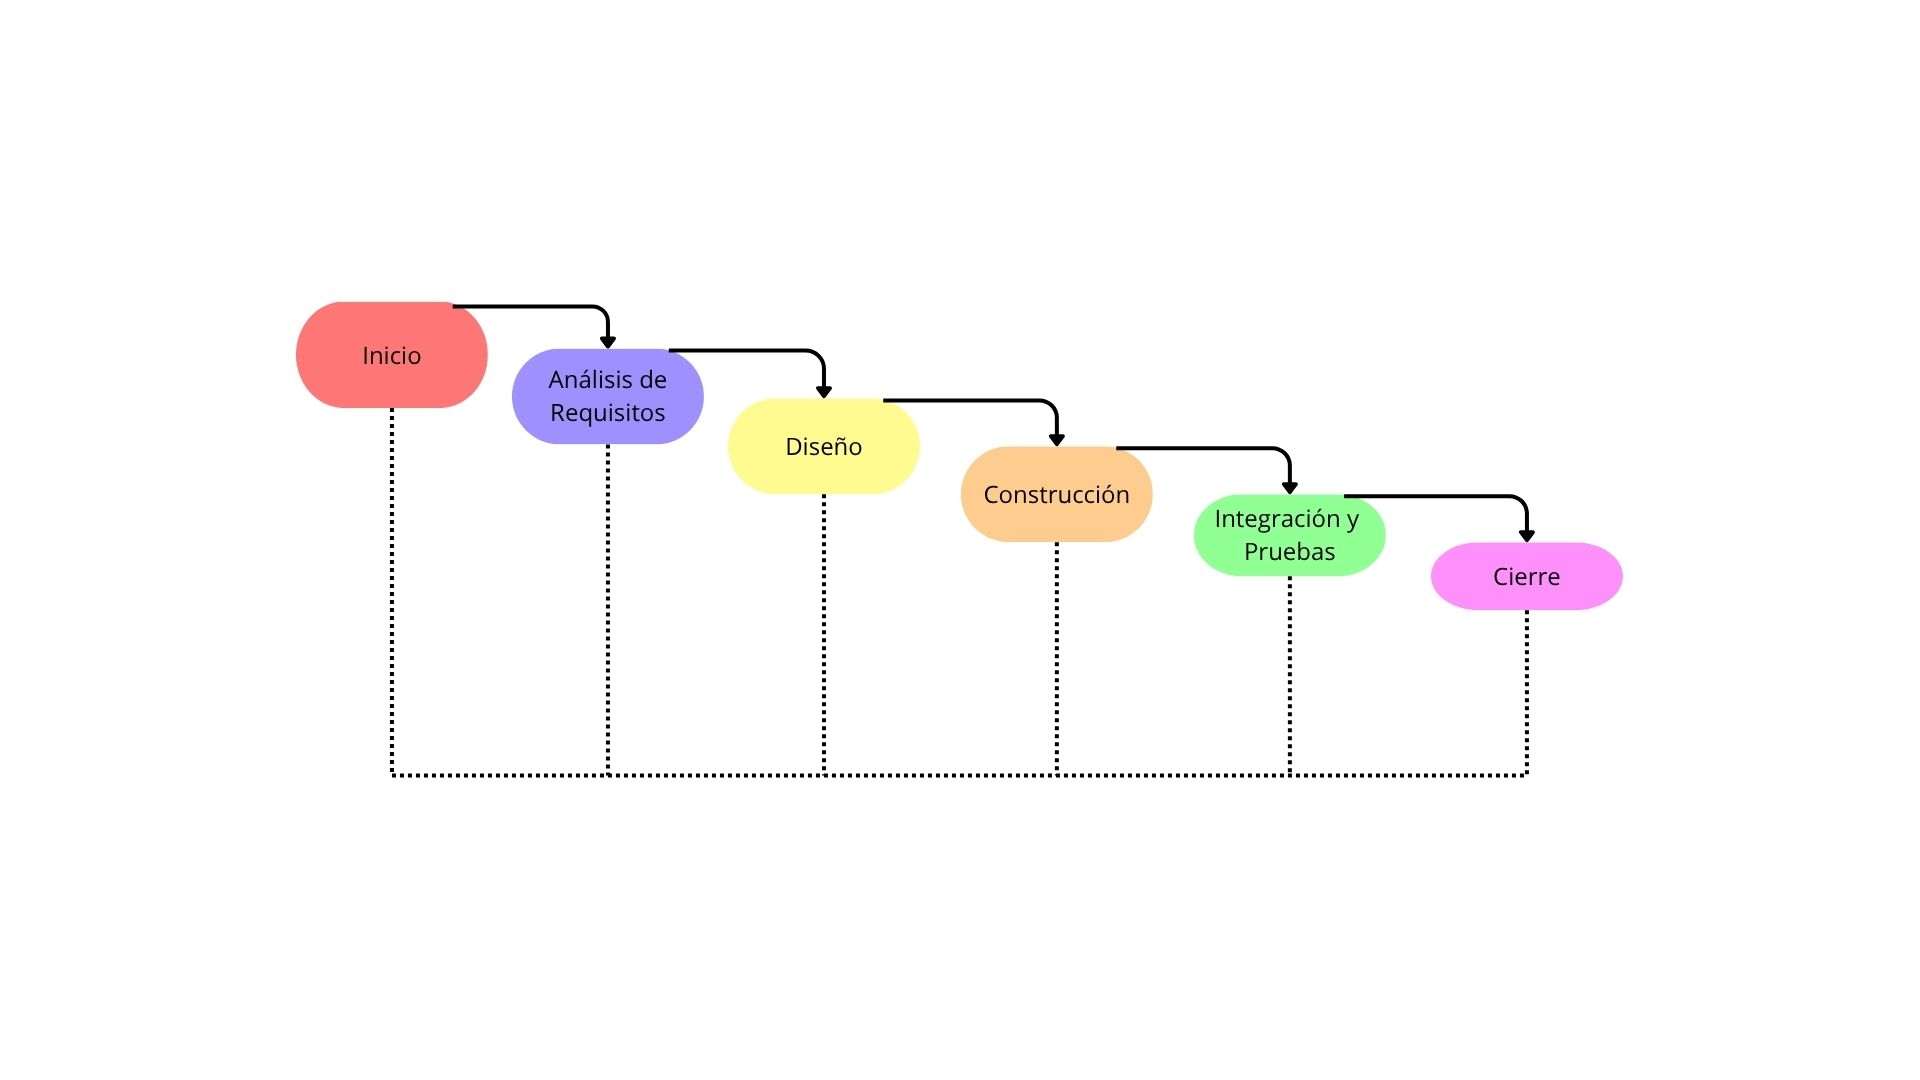
\includegraphics[width=1\linewidth]{figures/metodologia_desarrollo.jpg}
    \caption{Cascada iterativa (creación propia).}
    \label{fig:cascada}
\end{figure}


\section{Tecnologías}

Para este proyecto, se ha decidido hacer una aplicación multiplataforma, ya que se considera que al ser una aplicación dedicada tanto a aficionados como a analistas profesionales, era una buena práctica ofrecer al usuario una experiencia dedicada a su campo; si es un aficionado, la usará más en móvil, y si es un profesional, en ordenador. Además, el \textit{framework} usado nos permite implementar tanto para Android como para iOS con facilidad, así que también tendremos ese añadido.

En cuanto al diseño de la aplicación, podemos diferenciar \textit{frontend} y \textit{backend}. Además, se usa una tecnología como GitHub y GitHub Desktop, que nos permiten tener un control de versiones de la manera más eficiente y nos facilitan el desarrollo del proyecto y de sus cambios.

\subsection{\textit{Frontend}}

Para el desarrollo de la aplicación móvil se han tenido en cuenta tres tecnologías principales: Kotlin, React Native y Flutter. Todas ellas permiten desarrollar aplicaciones para dispositivos móviles, aunque presentan diferencias en cuanto a lenguaje utilizado, facilidad de desarrollo, rendimiento y experiencia previa del desarrollador.

En primer lugar, se valoró el uso de Kotlin. Kotlin es un lenguaje de programación moderno, conciso y de código abierto, desarrollado por \textit{JetBrains}, optimizado para la JVM, Android y el desarrollo multiplataforma. Destaca por su interoperabilidad con Java, su tipado estático, la seguridad frente a valores nulos y el soporte tanto para programación funcional como orientada a objetos. Aunque se contaba con experiencia previa en este lenguaje, los problemas de rendimiento encontrados con el emulador hicieron que se exploraran otras alternativas.

Otra opción considerada fue React Native. React Native es un \textit{framework} de código abierto creado por \textit{Facebook} para el desarrollo de aplicaciones móviles nativas para iOS y Android utilizando JavaScript y React. Esta opción resultaba especialmente atractiva al basarse en JavaScript, un lenguaje ya utilizado en proyectos anteriores, además de ser una tecnología ampliamente utilizada en el ámbito del desarrollo móvil.

Por último, también se tuvo en cuenta Flutter. Flutter es un \textit{framework} de código abierto desarrollado por \textit{Google} que permite crear aplicaciones compiladas de forma nativa y de alto rendimiento para dispositivos móviles, web y escritorio a partir de una única base de código. Se consideró una alternativa interesante por su enfoque multiplataforma, su rendimiento y su buena gestión de interfaces gráficas.

Finalmente, se decidió desarrollar la aplicación con React Native debido a la experiencia previa con JavaScript, la facilidad para realizar despliegues multiplataforma, la posibilidad de visualizar cambios en tiempo real durante el desarrollo y su alta demanda en el mercado laboral.

\subsection{\textit{Backend}}
Para la parte destinada a gestionar las peticiones que podrá realizar el usuario, se ha decidido emplear un conjunto de tecnologías que garanticen la persistencia, seguridad y eficiencia en el manejo de grandes volúmenes de datos.

\subsubsection{Base de datos}
Para la elección de la base de datos, primero se analizaron los dos paradigmas principales existentes en la actualidad: las bases de datos relacionales y las no relacionales (NoSQL).

Las bases de datos NoSQL ofrecen una gran flexibilidad y escalabilidad horizontal; sin embargo, para este proyecto se ha optado por una base de datos relacional. Esta decisión se basa en que los datos deportivos (jugadores, equipos, partidos y estadísticas) presentan una estructura tabular clara y relaciones estrictas entre ellos. El modelo relacional permite garantizar la integridad referencial mediante el uso de claves foráneas, asegurando que cada estadística esté correctamente vinculada a un jugador y un partido existentes, evitando así inconsistencias que podrían falsear los análisis posteriores.

\subsubsection{SGBD}
Como sistema gestor de bases de datos (SGBD) se ha seleccionado PostgreSQL. 

PostgreSQL es un sistema de código abierto objeto-relacional que destaca por su robustez, fiabilidad y por cumplir estrictamente con los estándares SQL. Su naturaleza \textit{open source} lo convierte en una opción idónea para proyectos académicos como el presente, ofreciendo prestaciones de nivel empresarial sin incurrir en costes de licenciamiento.

Para la administración y gestión de la base de datos se utilizará DBeaver. Esta herramienta de gestión universal permite interactuar con el servidor de forma visual y sencilla, facilitando tareas como la ejecución de consultas, el diseño de diagramas entidad-relación y la monitorización de los datos de manera intuitiva.

Durante la fase de planificación se consideraron otras alternativas, siendo MySQL la opción más destacada. Si bien MySQL es un gestor ampliamente utilizado, se eligió PostgreSQL debido a la experiencia previa en otros proyectos y, fundamentalmente, por las funciones avanzadas que ofrece este último (como su potencia en consultas analíticas), las cuales se adaptan mejor a los requisitos de procesamiento de datos de este trabajo.
\subsubsection{API}

Además de la base de datos y del SGBD, la aplicación necesita una API que sea capaz de gestionar las peticiones realizadas desde la aplicación móvil y proporcionar la funcionalidad necesaria sobre los datos almacenados. Para esta parte del sistema existen distintas tecnologías disponibles, aunque en este proyecto se han tenido en cuenta principalmente dos alternativas: Node.js y Python mediante FastAPI.

En primer lugar, una de las opciones consideradas ha sido Node.js. Node.js es un entorno de ejecución para JavaScript que permite ejecutar este lenguaje en el servidor, fuera del navegador. Está basado en el motor V8 de Google Chrome y destaca por su modelo de entrada/salida no bloqueante y orientado a eventos, lo cual lo hace adecuado para aplicaciones que requieren manejar varias conexiones al mismo tiempo, como \textit{chats}, APIs REST y servicios en tiempo real.

Por otro lado, también se ha valorado el uso de Python junto con FastAPI. Python es un lenguaje de programación interpretado, de alto nivel, conocido por su sintaxis clara y su legibilidad. En el desarrollo de APIs, Python es muy valorado por permitir escribir código rápidamente y con pocos errores, lo que lo hace adecuado para prototipado, ciencia de datos y aplicaciones basadas en inteligencia artificial. Para construir APIs en Python, uno de los \textit{frameworks} más utilizados actualmente es FastAPI.

Tras analizar ambas alternativas, se ha decidido utilizar Node.js, debido a que el desarrollador ya cuenta con experiencia previa en su uso dentro de otros proyectos académicos relacionados con la construcción de APIs. Además, al desarrollarse la aplicación móvil con React Native, el uso de Node.js en el \textit{backend} permite mantener una mayor coherencia en el lenguaje de programación empleado en el proyecto. Esto facilita la reutilización de conocimientos y agiliza el desarrollo al no tener que alternar entre diferentes sintaxis.

\subsubsection{Proceso ETL y \textit{data mining}}

Para la fase de procesamiento de datos y extracción de conocimiento, se ha seleccionado Python como lenguaje principal, debido a su versatilidad y a su ecosistema de librerías especializadas en ciencia de datos. Esta parte del sistema se divide en dos etapas fundamentales: el proceso ETL y la posterior aplicación de técnicas de \textit{data mining}.

En primer lugar, el proceso ETL (\textit{Extract, Transform, Load}) se encarga de preparar los datos antes de su carga definitiva en la base de datos. En esta fase se han desarrollado \textit{scripts} personalizados para la extracción de los datos en formato JSON procedentes de la API deportiva. Utilizando la librería Pandas, se realiza la limpieza y transformación de los datos, incluyendo la normalización de estructuras anidadas, la gestión de valores nulos y la corrección de tipos de datos, como la conversión de decimales innecesarios a enteros. Finalmente, los datos procesados se cargan de forma estructurada en la base de datos PostgreSQL.

Una vez consolidada la base de datos, se desarrolla la fase de \textit{data mining}. En esta etapa se aplican técnicas de minería de datos para descubrir patrones en el rendimiento de jugadores y equipos, generar indicadores y realizar predicciones. Python facilita la implementación de algoritmos de aprendizaje automático y análisis estadístico, permitiendo transformar los datos brutos en información de valor para el análisis deportivo.

La elección de Python se justifica por la potencia de herramientas como Pandas para la manipulación de grandes volúmenes de datos y Psycopg2 para la conexión eficiente con el servidor PostgreSQL.

\subsubsection{Asistente conversacional}

Para la implementación del asistente conversacional de la aplicación se ha utilizado Gemini, un modelo de inteligencia artificial generativa desarrollado por Google. Esta tecnología permite interpretar preguntas realizadas en lenguaje natural por el usuario y transformarlas en consultas sobre la información almacenada en el sistema.

El uso de Gemini se justifica por la necesidad de ofrecer una forma de consulta más flexible e intuitiva que la navegación tradicional por pantallas. A través del asistente, denominado Agente de oro, el usuario puede preguntar por estadísticas de jugadores, equipos, partidos o temporadas sin tener que acceder manualmente a cada apartado de la aplicación.

La integración se realiza desde el \textit{backend}, que actúa como intermediario entre la aplicación móvil, la base de datos y el modelo de inteligencia artificial. De esta forma, el usuario no interactúa directamente con el servicio externo, sino que las peticiones son controladas por la API, permitiendo limitar el tipo de consultas permitidas y garantizar que las respuestas se basen únicamente en la información deportiva disponible en la base de datos.

\subsubsection{Contenedorización y despliegue}

Para facilitar la ejecución del sistema en distintos entornos se ha considerado el uso de Docker. Docker permite empaquetar los diferentes servicios de la aplicación en contenedores independientes, asegurando que el backend, la base de datos y el resto de componentes se ejecuten con una configuración controlada y reproducible.

En este proyecto, la contenedorización resulta especialmente útil para simplificar la puesta en marcha del entorno de desarrollo y evitar problemas derivados de diferencias entre sistemas operativos, versiones de dependencias o configuraciones locales. Mediante un archivo de composición de servicios, es posible definir la base de datos PostgreSQL, el servidor backend y las variables de entorno necesarias para que la aplicación pueda ejecutarse de forma más sencilla en otra máquina.

Aunque el despliegue final en producción queda fuera del alcance principal del Trabajo Fin de Grado, Docker proporciona una base adecuada para una futura publicación del sistema, ya que permitiría trasladar el backend y la base de datos a un servidor externo manteniendo una configuración similar a la utilizada durante el desarrollo.

\section{Planificación del proyecto}
El diagrama de Gantt de la figura~\ref{fig:gantt} muestra el tiempo dedicado a desarrollar las diferentes partes del proyecto, empezando por el análisis de datos, diseño, implementación de arquitectura y aplicación, y acabando por la memoria. 
\begin{figure}[H]
    \centering
    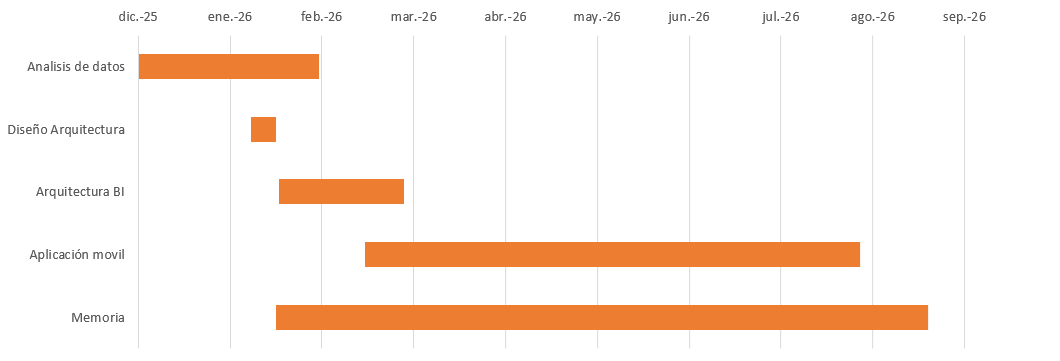
\includegraphics[width=1\linewidth]{figures/gantt_tfg.png}
    \caption{Diagrama de Gantt del proyecto.}
    \label{fig:gantt}
\end{figure}

\section{Costes}

En esta sección se presenta una estimación de los costes asociados al desarrollo del proyecto. Dado que se trata de un Trabajo Fin de Grado, muchos de los recursos utilizados ya estaban disponibles previamente o han sido empleados en un entorno académico, por lo que no todos han supuesto un coste económico directo. No obstante, se incluye una valoración aproximada del esfuerzo humano, los recursos materiales y los posibles costes de servicio en caso de que la aplicación quisiera desplegarse en un entorno de producción.

\subsection{Costes de recursos humanos}

El principal coste del proyecto corresponde al tiempo dedicado al análisis, diseño, desarrollo, pruebas y documentación del sistema. Aunque el trabajo ha sido realizado por un único desarrollador en el contexto académico del Trabajo Fin de Grado, se ha estimado su coste tomando como referencia una tarifa de 15 euros por hora, correspondiente a un perfil de desarrollador junior.

El periodo de desarrollo se ha extendido aproximadamente desde febrero hasta septiembre. Durante este periodo se estima que se ha trabajado en torno al 75 \% de los días, con una dedicación media aproximada de dos horas diarias. A partir de esta estimación, se obtiene un total de 363 horas de trabajo.

La Tabla~\ref{tab:costes_recursos_humanos} resume el coste estimado asociado a los recursos humanos.

\begin{table}[H]
\centering
\caption{Costes de recursos humanos.}
\label{tab:costes_recursos_humanos}
\renewcommand{\arraystretch}{1.2}
\begin{tabular}{|p{5cm}|p{4cm}|p{4cm}|}
\hline
\textbf{Concepto} & \textbf{Cantidad} & \textbf{Coste estimado} \\ \hline

Periodo de desarrollo &
Febrero - septiembre &
- \\ \hline

Dedicación estimada &
363 horas &
- \\ \hline

Coste por hora &
15 \euro/hora &
- \\ \hline

Desarrollo del proyecto &
363 horas &
5.445 \euro \\ \hline

\textbf{Total recursos humanos} &
&
\textbf{5.445 \euro} \\ \hline

\end{tabular}
\end{table}

\subsection{Costes materiales}

Los costes materiales corresponden a los recursos físicos y de soporte utilizados durante el desarrollo del proyecto. En este caso, se ha utilizado un ordenador portátil personal y un dispositivo móvil físico para realizar pruebas de la aplicación. Al tratarse de recursos ya disponibles antes del inicio del proyecto, no se ha imputado un coste directo asociado a su adquisición.

Además, se han considerado otros recursos necesarios para el desarrollo, como la conexión a Internet y el consumo eléctrico. Aunque estos recursos forman parte del entorno doméstico habitual, se incluye una estimación proporcional asociada al tiempo dedicado al proyecto. Para la electricidad, se ha estimado el consumo aproximado del ordenador portátil durante las horas de trabajo. Para la conexión a Internet, se ha considerado una parte proporcional del uso durante los meses de desarrollo.

La Tabla~\ref{tab:costes_materiales} recoge los principales costes materiales considerados.

\begin{table}[H]
\centering
\caption{Costes materiales.}
\label{tab:costes_materiales}
\renewcommand{\arraystretch}{1.2}
\begin{tabular}{|p{6cm}|p{5cm}|p{3cm}|}
\hline
\textbf{Recurso} & \textbf{Descripción} & \textbf{Coste} \\ \hline

Ordenador portátil &
Recurso personal ya disponible &
0 \euro \\ \hline

Dispositivo móvil &
Recurso personal utilizado para pruebas &
0 \euro \\ \hline

Conexión a Internet &
Uso proporcional de la red doméstica durante el desarrollo del proyecto &
40 \euro \\ \hline

Consumo eléctrico &
Estimación del consumo del equipo durante las horas de desarrollo &
5 \euro \\ \hline

\textbf{Total costes materiales} &
&
\textbf{45 \euro} \\ \hline

\end{tabular}
\end{table}

\subsection{Costes de servicios}

Durante el desarrollo del proyecto se ha utilizado la API-Football durante un mes para obtener datos históricos y actuales de la competición. Este servicio ha supuesto un coste directo de 30 euros. Por otro lado, el asistente inteligente se ha apoyado en Google AI Studio, disponible de forma gratuita mediante el entorno universitario, por lo que no se ha considerado coste asociado a este servicio dentro del desarrollo académico.

La Tabla~\ref{tab:costes_servicios_desarrollo} muestra los costes de servicios utilizados durante el desarrollo.

\begin{table}[H]
\centering
\caption{Costes de servicios durante el desarrollo.}
\label{tab:costes_servicios_desarrollo}
\renewcommand{\arraystretch}{1.2}
\begin{tabular}{|p{6cm}|p{6cm}|p{3cm}|}
\hline
\textbf{Servicio} & \textbf{Uso en el proyecto} & \textbf{Coste} \\ \hline

API-Football &
Obtención de datos históricos y actuales de LaLiga durante un mes &
30 \euro \\ \hline

Google AI Studio &
Servicio utilizado para el asistente conversacional en entorno académico &
0 \euro \\ \hline

\textbf{Total servicios de desarrollo} &
&
\textbf{30 \euro} \\ \hline

\end{tabular}
\end{table}

Además de los costes reales del desarrollo, se puede considerar un escenario hipotético de puesta en producción. En dicho caso, la aplicación requeriría una infraestructura adicional para alojar el backend, la base de datos, los servicios de inteligencia artificial y el consumo recurrente de una API deportiva. Estos costes no forman parte del coste real del Trabajo Fin de Grado, pero permiten estimar la inversión necesaria si el sistema quisiera desplegarse para usuarios reales.

La Tabla~\ref{tab:costes_produccion} presenta una estimación mensual para un posible despliegue en producción.

\begin{table}[H]
\centering
\caption{Estimación de costes mensuales en un escenario de producción.}
\label{tab:costes_produccion}
\renewcommand{\arraystretch}{1.2}
\begin{tabular}{|p{6cm}|p{6cm}|p{3cm}|}
\hline
\textbf{Servicio} & \textbf{Descripción} & \textbf{Coste mensual estimado} \\ \hline

Servidor backend &
Alojamiento de la API REST desarrollada en Node.js &
10--20 \euro \\ \hline

Base de datos PostgreSQL &
Servicio gestionado o servidor con PostgreSQL desplegado &
15--30 \euro \\ \hline

API de datos deportivos &
Obtención periódica o en tiempo real de datos de partidos, equipos y jugadores &
30--100 \euro \\ \hline

Servicio de inteligencia artificial &
Uso de un modelo de lenguaje para el asistente conversacional &
0--30 \euro \\ \hline

Dominio y certificado SSL &
Dominio web y seguridad HTTPS básica &
1--5 \euro \\ \hline

Monitorización y copias de seguridad &
Control básico del estado del sistema y respaldo de datos &
5--15 \euro \\ \hline

\textbf{Total mensual estimado} &
&
\textbf{61--200 \euro/mes} \\ \hline

\end{tabular}
\end{table}

Esta estimación dependería del número de usuarios, la frecuencia de actualización de los datos, el volumen de consultas realizadas al asistente inteligente y el nivel de disponibilidad requerido. Por tanto, debe entenderse como una aproximación inicial para un despliegue básico, no como un presupuesto cerrado de explotación comercial.

\subsection{Coste total estimado}

Teniendo en cuenta los costes reales asociados al desarrollo académico del proyecto, el coste total estimado se obtiene sumando el coste de recursos humanos, los costes materiales y los servicios utilizados durante el desarrollo.

La Tabla~\ref{tab:coste_total_proyecto} recoge el coste total estimado del proyecto.

\begin{table}[H]
\centering
\caption{Coste total estimado del proyecto.}
\label{tab:coste_total_proyecto}
\renewcommand{\arraystretch}{1.2}
\begin{tabular}{|p{8cm}|p{4cm}|}
\hline
\textbf{Concepto} & \textbf{Coste} \\ \hline

Costes de recursos humanos &
5.445 \euro \\ \hline

Costes materiales &
45 \euro \\ \hline

Costes de servicios durante el desarrollo &
30 \euro \\ \hline

\textbf{Coste total estimado del proyecto} &
\textbf{5.520 \euro} \\ \hline

\end{tabular}
\end{table}

Por tanto, el coste estimado del desarrollo del proyecto asciende a 5.520 euros. Este valor representa una estimación económica del esfuerzo y los recursos empleados durante el Trabajo Fin de Grado, aunque el coste real asumido ha sido menor al haberse utilizado principalmente recursos personales, herramientas gratuitas y servicios académicos.
\section{Riesgos}
Para poder anticipar obstáculos y posibles errores que tengamos que solucionar, es fundamental identificar los posibles riesgos que podamos encontrar por el camino. Estos serían los principales riesgos que podemos encontrar:
\begin{itemize}
    \item Cambios en los requisitos: durante el proceso, podemos encontrar dificultades en algunas funcionalidades o plataformas usadas que pueden desencadenar retrasos o modificaciones.
    \item Curva de aprendizaje: podemos encontrar dificultades para aprender a usar una tecnología o lenguaje que nunca se haya usado, y tener que ralentizar para dominarla.
    \item Rango de datos limitado: por falta de financiación para una API de datos futbolísticos avanzada, quizás los datos recogidos no sean lo más completos posible para hacer los análisis.
    \item \textit{Hardware} y recursos de pruebas: el desarrollo de aplicación móvil conlleva tener un \textit{hardware} que sea capaz de ejecutar la app para la toma de pruebas.
    \item Compatibilidad entre plataformas: podemos tener dificultades en la portabilidad de la aplicación hacia Android o iOS.
\end{itemize}

